\documentclass[aspectratio=169,12pt]{beamer}
\usepackage[utf8]{inputenc}
\usepackage[spanish, es-nodecimaldot]{babel}
%\usepackage{icomma} % Use dot as decimal separator
\usepackage{booktabs} % For better-looking tables
\usepackage{wrapfig}
\usepackage{caption}
%\usepackage{siunitx}


\usepackage{refcount}

\usepackage{enumitem}

\usepackage{multicol}
\usepackage{mathtools}

\usepackage[normalem]{ulem}

\pagestyle{empty}

\usepackage{pgf,tikz}
\usepackage{pgfplots}
\usetikzlibrary{matrix}
\usetikzlibrary{arrows}

%\usepackage{wrapfig}
\mode<presentation>
\usefonttheme{professionalfonts}
\usetheme{Darmstadt}
\usecolortheme{orchid}
\useoutertheme{default}
\setbeamertemplate{headline}{}

\renewcommand{\baselinestretch}{1.1}

%gets rid of bottom navigation bars
\setbeamertemplate{footline}[page number]

%gets rid of navigation symbols
\setbeamertemplate{navigation symbols}{}

%\frameframe{none} % No default frame

%\setlength{\framewidth}{8.7in} \setlength{\frameheight}{7.2in}

\parindent 0pt
\setlength{\parskip} {1ex plus 0.5ex minus 0.2ex}


%\usepackage[bbgreekl]{mathbbol}
\usepackage{amsfonts}

%\DeclareSymbolFontAlphabet{\mathbb}{AMSb}
%\DeclareSymbolFontAlphabet{\mathbbl}{bbold}

\newcommand{\Sym}{{\mathcal S}}
\DeclareMathOperator{\Aut}{Aut}
\DeclareMathOperator{\Tr}{Tr}
\DeclareMathOperator{\trace}{Trace}
\DeclareMathOperator{\range}{range}
\DeclareMathOperator{\rank}{rank}

\usepackage{breqn}
\usepackage{multicol}
\usepackage{colortbl}
\usepackage{lmodern}
\usepackage{tabularx}
\usepackage{multirow}
\usepackage{amssymb}
\usepackage{amsmath}
\usepackage{stmaryrd}
\usepackage{color}
\usepackage{graphicx}
\graphicspath{ {img/} }
\usepackage{hyperref}

\input{epsf}
\title{Introducción}
\author{}

\DeclareMathOperator{\Hom}{Hom}
\DeclareMathOperator{\sing}{sing}

\DeclareMathOperator{\chara}{char}
\DeclareMathOperator{\Jacob}{Jacob}
\DeclareMathOperator{\Sing}{Sing}
\newcommand{\fracNoLine}[2]{\genfrac{}{}{}{0pt}{#1}{#2}}

%\beamerdefaultoverlayspecification{<+->}

\usepackage{listings,xcolor,bm}


\definecolor{mygreen}{rgb}{0,0.6,0}
\definecolor{mygray}{rgb}{0.5,0.5,0.5}
\definecolor{mymauve}{rgb}{0.58,0,0.82}
\lstset{
  backgroundcolor=\color{white},   % choose the background color; you must add
  basicstyle=\small\ttfamily,      % the size of the fonts that are used for the code
  breakatwhitespace=false,         % sets if automatic breaks should only happen at whitespace
  breaklines=true,                 % sets automatic line breaking
  captionpos=b,                    % sets the caption-position to bottom
  commentstyle=\color{mygreen},    % comment style
  deletekeywords={...},            % if you want to delete keywords from the given language
  escapeinside={\%*}{*)},          % if you want to add LaTeX within your code
  extendedchars=true,              % lets you use non-ASCII characters; for 8-bits encodings only, does not work with UTF-8
  firstnumber=1,                % start line enumeration with line 1000
  frame=single,	                   % adds a frame around the code
  keepspaces=true,                 % keeps spaces in text, useful for keeping indentation of code (possibly needs columns=flexible)
  keywordstyle=\color{blue},       % keyword style
  language=Python,                 % the language of the code
  morekeywords={*,...},            % if you want to add more keywords to the set
  numbers=left,                    % where to put the line-numbers; possible values are (none, left, right)
  numbersep=5pt,                   % how far the line-numbers are from the code
  numberstyle=\tiny\color{mygray}, % the style that is used for the line-numbers
  rulecolor=\color{black},         % if not set, the frame-color may be changed on line-breaks within not-black text (e.g. comments (green here))
  showspaces=false,                % show spaces everywhere adding particular underscores; it overrides 'showstringspaces'
  showstringspaces=false,          % underline spaces within strings only
  showtabs=false,                  % show tabs within strings adding particular underscores
  stepnumber=5,                    % the step between two line-numbers. If it's 1, each line will be numbered
  stringstyle=\color{mymauve},     % string literal style
  tabsize=4,	                   % sets default tabsize to 2 spaces
  title=\lstname                   % show the filename of files included with \lstinputlisting; also try caption instead of title
}

\begin{document}

\newtheorem{prop}{Proposici\'on}
\newtheorem{algo}[prop]{Algorithm}
\newtheorem{teor}[prop]{Theorem}
\newtheorem{lema}[prop]{Lemma}
\newtheorem{coro}[prop]{Corollary}
\newtheorem{defi}[prop]{Definition}

\newcommand{\ideal}[1]{{\left\langle{#1}\right\rangle}}
\newcommand{\demo}{\textbf {Demostraci\'on. }}
\newcommand{\obse}{\textbf {Observaci\'on. }}
\newcommand{\Input}{\textbf {Input: }}
\newcommand{\Output}{\textbf {Output: }}
\newcommand{\Examp}{\textbf {Ejemplo }}
\newcommand{\Examps}{\textbf {Ejemplos }}

\newcommand{\kk}{{\mathbbl k}}
\newcommand{\V}{{\mathbf V}}
\newcommand{\I}{{\mathbf I}}
\newcommand{\PP}{{\tilde P}}
\newcommand{\QQ}{{\tilde Q}}

\newcommand{\F}{{\mathbb F}}
\newcommand{\Q}{{\mathbb Q}}
\newcommand{\N}{{\mathbb N}}
\newcommand{\R}{{\mathbb R}}
\newcommand{\Z}{{\mathbb Z}}
\newcommand{\CC}{{\mathbb C}}
\newcommand{\eLL}{{\mathcal L}}



\newcommand{\MinAss}{\textrm {MinAss}}
\newcommand{\Ass}{\textrm {Ass}}
\newcommand{\mcm}{\textrm {mcm}}
\newcommand{\mcd}{\textrm {mcd}}
%\newcommand{\mod}{\textrm { mod }}
\newcommand{\lt}{\textrm {lt}}
\newcommand{\Lt}{\textrm {Lt}}
\newcommand{\lp}{\textrm {lp}}
\newcommand{\lc}{\textrm {lc}}
\newcommand{\lm}{\textrm {lm}}
\newcommand{\barra}{\ /\ }
\newcommand{\multideg}{\textrm {multideg}}

\newcommand{\sep}{\textrm {sep}}
\newcommand{\Syz}{\textrm {Syz}}
\newcommand{\n}{\~n}
\newcommand{\cG}{\textrm {cG}}
\newcommand{\dG}{\textrm {dG}}
\newcommand{\nG}{\textrm {nG}}
\newcommand{\CE}{\textrm {CE}}
\newcommand{\CG}{\textrm {CG}}
\newcommand{\CF}{\textrm {CF}}
\newcommand{\DG}{\textrm {DG}}
\renewcommand{\NG}{\textrm {NG}}

\newcommand{\p}{{\boldsymbol{p}}}
\newcommand{\q}{{\boldsymbol{q}}}

\newcommand{\X}{{\boldsymbol{X}}}
\newcommand{\x}{{\boldsymbol{x}}}
\renewcommand{\u}{{\boldsymbol{u}}}
\renewcommand{\t}{{\boldsymbol{t}}}
\renewcommand{\a}{{\boldsymbol{a}}}
\renewcommand{\b}{{\boldsymbol{b}}}
\renewcommand{\c}{{\boldsymbol{c}}}

%Titulos en espa�ol
%\renewcommand{\chaptername}{Cap\'{\i}tulo}
%\renewcommand{\bibname}{Bibliograf\'{\i}a}

\newcommand{\kring}{\kk[\x]}
\newcommand{\kRing}{\kk[X]}
\newcommand{\qring}{\Q[\x]}

%\renewcommand\itemindent{-10pt}
%\renewcommand{\theenumi}{\arabic{enumi}}
%\renewcommand{\labelenumi}{\Alph{enumi}}

\definecolor{issac}{rgb}{1.00,0.00,0.00}
%------------------------------------------------------------------

\begin{frame}

 \begin{center}

\Large\textbf{Laboratorio de Datos} \\
\large\textbf{Clustering: DBSCAN}
%\vspace{0.5cm}

% \textit{Santiago Laplagne} \\
%slaplagn@dm.uba.ar \\


%\vspace{0.5cm}
%{\small Trabajo en progreso en conjunto con \emph{Jose Capco} (Universit\"at Innsbruck) y \emph{Claus Scheiderer} %(Universit\"at Konstanz).} \\

\vspace{1cm}
Primer Cuatrimestre 2024 \\ Turnos tarde y noche

\vspace{1cm}


 {\small Facultad de Ciencias Exactas y Naturales, UBA}
 \end{center}


\end{frame}

%------------------------------------------------------------------

\begin{frame}
\frametitle{Repaso}

\textbf{Aprendizaje no supervisado}
\begin{itemize}
    \item El objetivo es encontrar patrones o estructuras ocultas en los datos.
    \item No conocemos o no hay a priori una respuesta correcta.
    \item Ejemplos: agrupación (clustering), reducción de dimensionalidad.
\end{itemize}

\textbf{Clustering}
\begin{itemize}
\item El objetivo es agrupar datos similares en conjuntos llamados clústeres.
\item Aplicaciones: segmentación de mercado, análisis de redes sociales, imagenes médica, etc.
\end{itemize}

\end{frame}

%------------------------------------------------------------------

\begin{frame}
\frametitle{Repaso: $k$-medias}

\begin{minipage}{.6\textwidth}
\begin{itemize}
    \item $K$-medias es un algoritmo de agrupación que particiona los datos en $k$ clústeres.
    \item Se definen $k$ centros para los clusters.
    \item Se supone que cada cluster es un conjunto de datos que están razonablemente bien aproximados por el centro del cluster (el promedio de los valores del cluster).
\end{itemize}


\textbf{Requerimiento importante:} los clusters deben ser esféricos e isotrópicos (el mismo radio en todas las direcciones).

$K$-medias no funciona bien si los clusters tienen formas irregulares.

\end{minipage}%
\begin{minipage}{.4\textwidth}

    \begin{center}
    
\includegraphics[scale=0.05]{clash-fingerUp.png}

    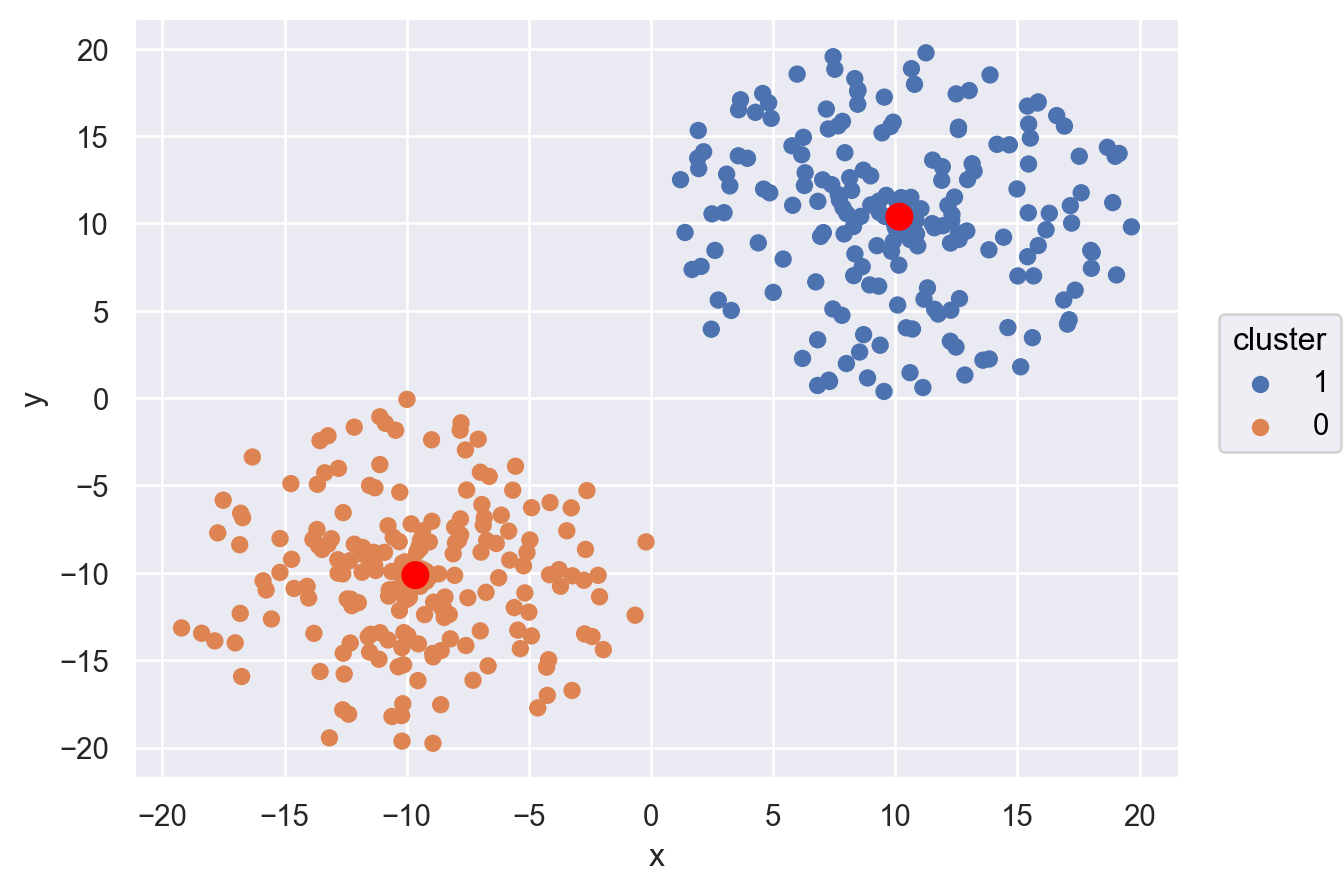
\includegraphics[scale=0.25]{clase15-convexblobs-etiquetado.png}

    
\includegraphics[scale=0.05]{clash-sad.png}

    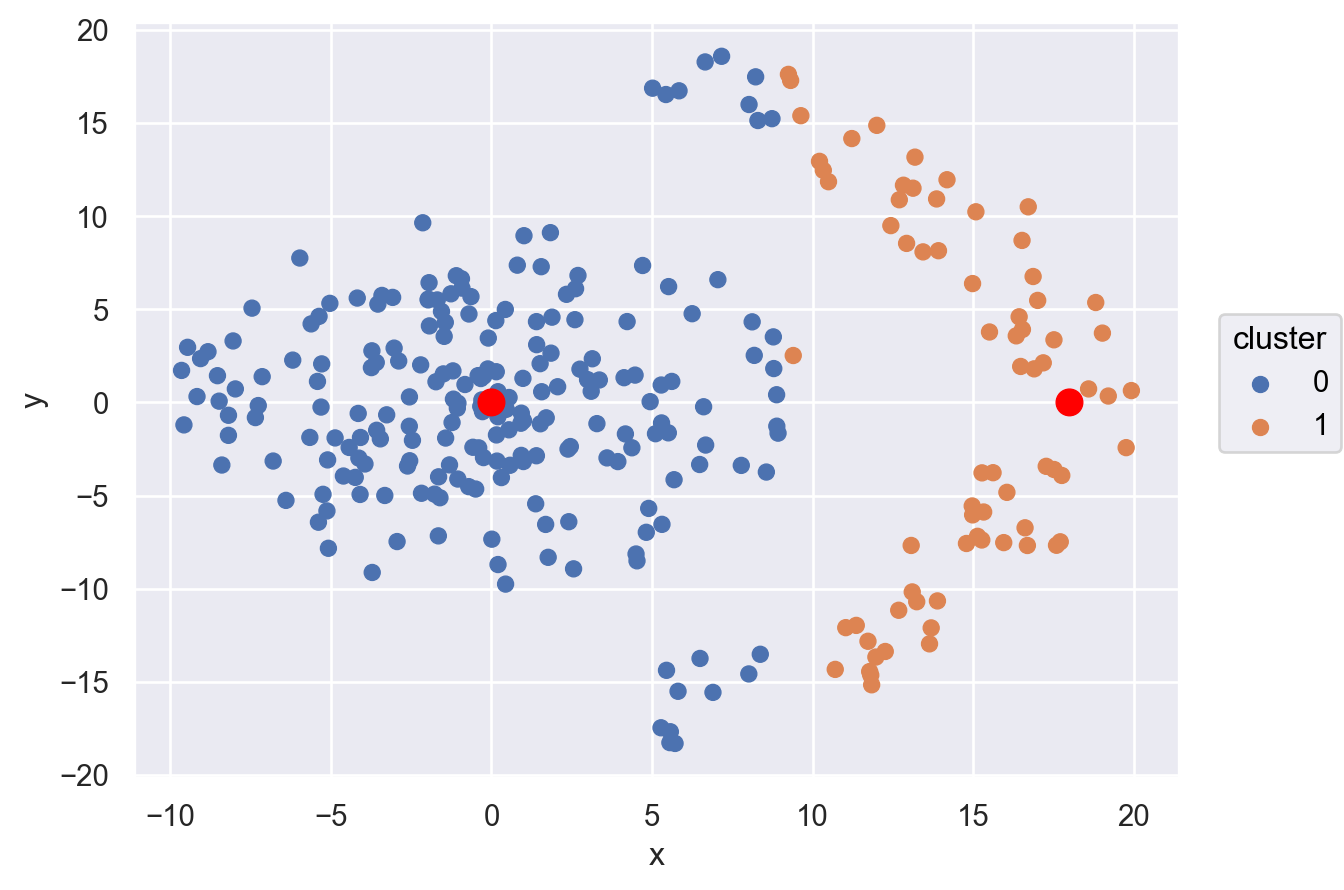
\includegraphics[scale=0.25]{clase15-nonconvexblobs-etiquetado.png}
    \end{center}
\end{minipage}

\end{frame}

%------------------------------------------------------------------

\begin{frame}
\frametitle{DBSCAN}

\begin{minipage}{.6\textwidth}
DBSSCAN es ``Density-based spatial clustering of applications with noise'' (agrupamiento espacial de aplicaciones con ruido basado en densidad)

\begin{itemize}
\item Dado un conjunto de puntos en el espacio, se agrupan puntos que están muy juntos (puntos con muchos puntos vecinos).
\item Se marcan como valores atípicos (outliers) puntos que se encuentran solos en regiones de baja densidad.
\end{itemize}

\end{minipage}%
\begin{minipage}{.4\textwidth}
    \begin{center}
    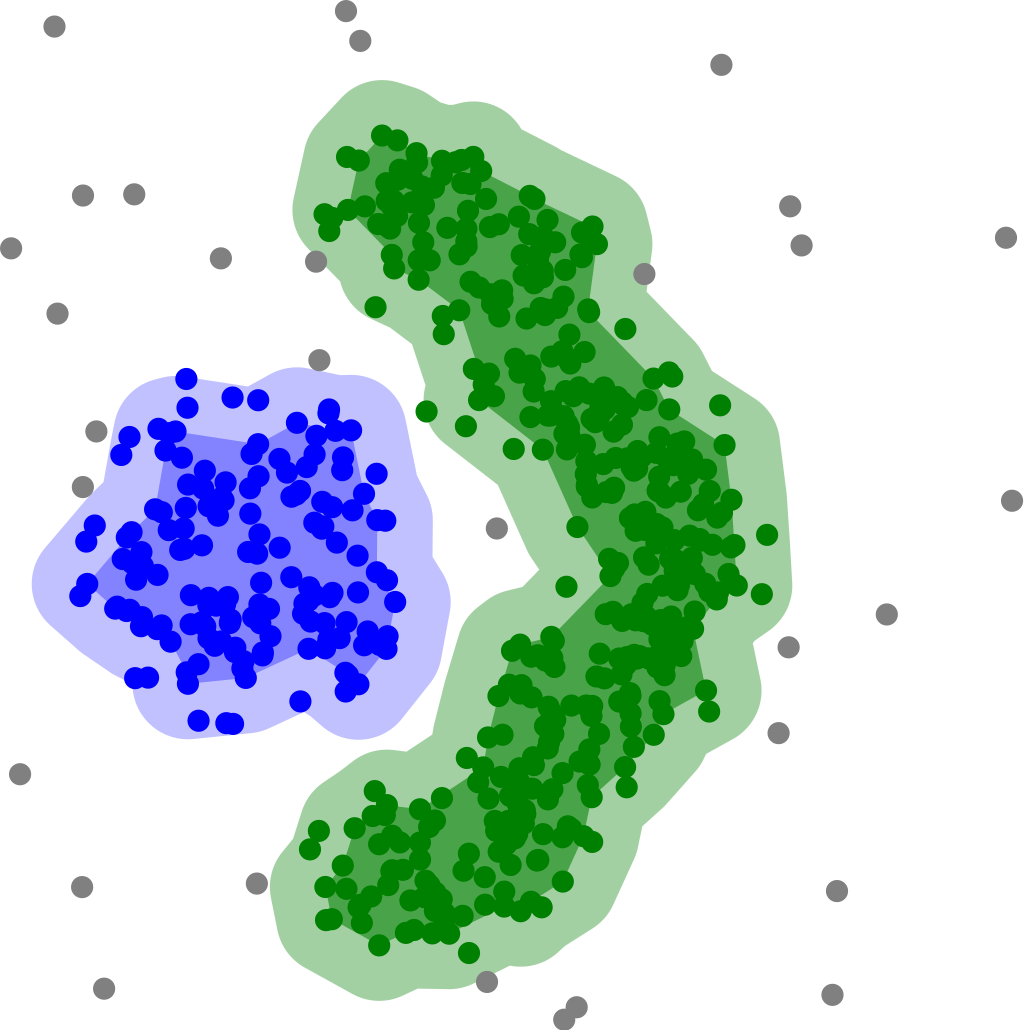
\includegraphics[scale=0.12]{clase16-DBSCAN-density-data.png}
    \end{center}
\end{minipage}

\end{frame}

%------------------------------------------------------------------

\begin{frame}
\frametitle{DBSCAN}

DBSCAN depende de dos parámetros:
\begin{itemize}
\item Un radio $\varepsilon$ (epsilon)
\item Un valor $minPts$ que indica cuandos puntos se espera encontrar en la vecindad de un punto de un cluster.
\end{itemize}

\begin{minipage}{.7\textwidth}
Utilizando esos parámetros, los datos se clasifican en
\begin{enumerate}
\item Puntos \emph{centrales} $p$.
\item Puntos \emph{directamente alcanzables} $q$ desde un punto central $p$.
\item Punto $q$ \emph{alcanzables} desde un punto central $p$.
\item Puntos \emph{atípicos}, todos los puntos que no son alcanzables desde ningún punto central.
\end{enumerate}
\end{minipage}%
\begin{minipage}{.3\textwidth}
    \begin{center}
    \includegraphics[scale=0.22]{clase16-DBSCAN-illustration.png}
    \end{center}
\end{minipage}


\end{frame}

%------------------------------------------------------------------

\begin{frame}
\frametitle{DBSCAN - Definiciones}

\begin{minipage}{.7\textwidth}
Concretamente, a partir de $\varepsilon$ y $minPts$ definimos:

\begin{enumerate}
\item Puntos \emph{centrales} $p$, si al menos $minPts$ puntos están a una distancia $\varepsilon$ de $p$ (incluido $p$).
\item Puntos \emph{directamente alcanzables} $q$ desde un punto central $p$, si $q$ está a distancia menor o igual que $\varepsilon$ de un punto central $p$.
\item Puntos $q$ \emph{alcanzables} desde $p$ si hay un camino $p_1, \dots, p_n$ con $p_1 = p$ y $p_n = q$, donde cada $p_{i+1}$ es directamente alcanzable desde $p_i$.
\item Puntos \emph{atípicos}, todos los puntos que no son alcanzables desde ningún punto central.
\end{enumerate}
\end{minipage}%
\begin{minipage}{.3\textwidth}
    \begin{center}
    \includegraphics[scale=0.22]{clase16-DBSCAN-illustration.png}
    \end{center}
\end{minipage}

\end{frame}

%------------------------------------------------------------------


\begin{frame}
\frametitle{Puntos centrales y puntos bordes}

\begin{minipage}{.6\textwidth}
Cada cluster queda compuesto por 
\begin{itemize}
\item puntos centrales
\item puntos alcanzables desde un punto central que no son centrales, estos puntos se denominan puntos frontera.
\end{itemize}

En el gráfico vemos la región central (puntos del plano que tienen al menos $minPts$ vecinos) y la región borde (puntos del plano con menos de $minPts$ vecinos alcanzables desde un punto central ).
\end{minipage}%
\begin{minipage}{.4\textwidth}
    \begin{center}
    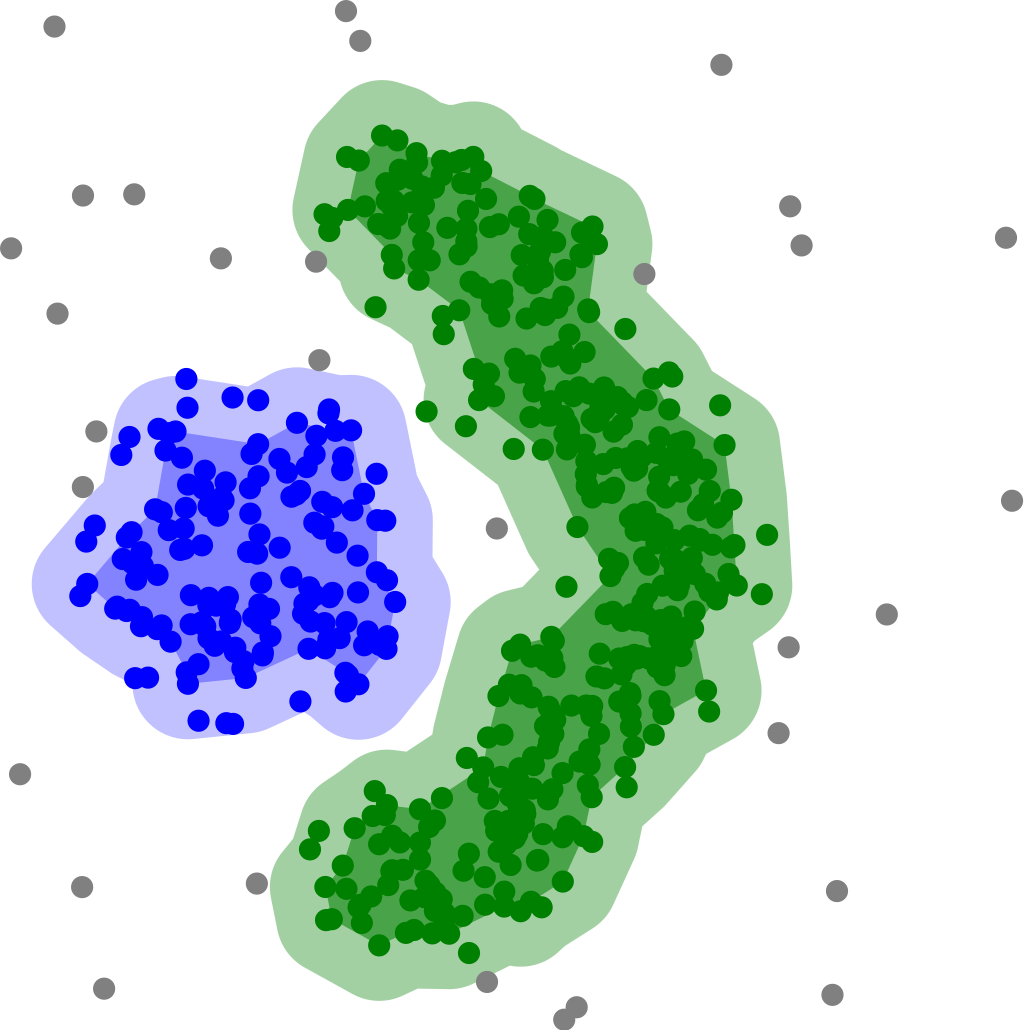
\includegraphics[scale=0.12]{clase16-DBSCAN-density-data.png}
    \end{center}
\end{minipage}

\end{frame}

%------------------------------------------------------------------


\begin{frame}
\frametitle{Algoritmo para construir un cluster}

El cluster asociado a un punto central $p$ está constituido por todos los puntos alcanzables desde $p$.

Obtenemos el siguiente algoritmo para construir un cluster a partir de un punto central:
\begin{enumerate}
\item Identificamos un punto central $p$ (que no pertenezca a ningún cluster ya construido).
\item Agregamos al cluster a todos los puntos $q$ directamente alcanzables desde $p$.
\item Si agregamos puntos centrales nuevos al cluster, agregamos al cluster a todos los puntos alcanzables desde los nuevos puntos centrales.
\item Repetimos el Paso 3 hasta que no hayamos agregado ningún nuevo punto al cluster.
\end{enumerate}

\end{frame}

%------------------------------------------------------------------

\begin{frame}
\frametitle{Ejemplo: construir el cluster asociado al punto central $p$}

Tomamos $\varepsilon = 1$ (radios utilizados en el gráfico) y minPts = 4.

\begin{enumerate}
\item $p$ es un punto central
\item Añadimos al cluster los 3 puntos directamente alcanzables desde $p$.
\item Solo uno de esos 3 puntos es un punto central.
\item Añadimos al cluster los 2 puntos alcanzables desde ese nuevo punto central.
\item No añadimos ningún nuevo punto central, por lo tanto finalizamos.
\end{enumerate}


\begin{tikzpicture}
    \fill[red] (8,8) circle (2pt);
    \draw[black, thin] (8,8) circle (.5);
    \node[anchor=south] at (8,8) {{\tiny $p$}};
    \fill[red] (8.2,8.4) circle (2pt);
    \draw[black, thin] (8.2,8.4) circle (.5);
    \fill[red] (7.8,7.6) circle (2pt);
    \draw[black, thin] (7.8,7.6) circle (.5);
    \fill[red] (8.4,7.8) circle (2pt);
    \draw[black, thin] (8.4,7.8) circle (.5);
    \fill[red] (7.4,7.5) circle (2pt);
    \draw[black, thin] (7.4,7.5) circle (.5);
    \fill[red] (7.9,7.2) circle (2pt);
    \draw[black, thin] (7.9,7.2) circle (.5);
    \fill[red] (7,7.5) circle (2pt);
    \draw[black, thin] (7,7.5) circle (.5);
    \fill[red] (7,8.2) circle (2pt);
    \draw[black, thin] (7,8.2) circle (.5);
\end{tikzpicture}

\end{frame}

%------------------------------------------------------------------


\begin{frame}
\frametitle{Algoritmo DBSCAN}

Comenzamos con un conjunto de puntos sin etiquetar.

\begin{enumerate}
\item Seleccionamos un punto central $P$ no etiquetado y le asignamos un nuevo cluster.
\item Construimos el cluster asociado a $P$ como vimos antes y les asignamos a todos los puntos la etiqueta correspondiente al cluster.
\item Repetimos los puntos 1 y 2 hasta que no haya ningún punto central no etiquetado.
\item Todos los puntos que quedaron sin etiquetar, los etiquetamos como valores atípicos.
\end{enumerate}

Nota: los puntos frontera pueden quedar asignados a clusters distintos según el orden en que etiquetamos, pero los puntos centrales en cada cluster son siempre los mismos.

\end{frame}

\begin{frame}{Comparación de K-means y DBSCAN}
    \begin{columns}
        \column{0.5\textwidth}
        \begin{block}{K-means}
{\footnotesize
                Método de Clustering: Basado en particiones

                Supuestos:
                    \begin{itemize}[noitemsep,nolistsep]
                        \item Los datos son esféricos o isotrópicos
                        \item Los clusters tienen tamaños similares
                    \end{itemize}

                Fortalezas:
                    \begin{itemize}[noitemsep,nolistsep]
                        \item Simple y rápido
                        \item Funciona bien con grandes conjuntos de datos
                    \end{itemize}

                Debilidades:
                    \begin{itemize}[noitemsep,nolistsep]
                        \item Requiere pre-especificar K
                        \item Sensible a la inicialización
                        \item Desempeño pobre con clusters no globulares
                    \end{itemize}
}
        \end{block}

        \column{0.5\textwidth}
        \begin{block}{DBSCAN}
        {\footnotesize
                Método de Clustering: Basado en densidad

                Supuestos:
                    \begin{itemize}[noitemsep,nolistsep]
                        \item Los clusters son regiones densas en el espacio de datos
                    \end{itemize}

                Fortalezas:
                    \begin{itemize}[noitemsep,nolistsep]
                        \item Puede encontrar clusters de formas arbitrarias
                        \item No necesita especificar el número de clusters
                        \item Robusto a valores atípicos (outliers)
                    \end{itemize}

                Debilidades:
                    \begin{itemize}[noitemsep,nolistsep]
                        \item Requiere establecer $\varepsilon$ y minPts
                        \item Desempeño pobre con densidad variable
                    \end{itemize}
}
        \end{block}
    \end{columns}
\end{frame}
\end{document}

%------------------------------------------------------------------

\begin{frame}[fragile]
\frametitle{Aplicación de K-means en Python}
\begin{itemize}
    \item Ejemplo de implementación en Python usando \texttt{scikit-learn}:
\end{itemize}

\begin{lstlisting}
from sklearn.cluster import KMeans
import numpy as np

# Datos de ejemplo
X = np.array([[1, 2], [1, 4], [1, 0],
              [10, 2], [10, 4], [10, 0]])

# Inicializar K-means
kmeans = KMeans(n_clusters=2, random_state=0).fit(X)

# Resultados
print(kmeans.labels_)
print(kmeans.cluster_centers_)
\end{lstlisting}

\end{frame}



\begin{frame}{Comparison of K-means and DBSCAN}
    \begin{columns}
        \column{0.5\textwidth}
        \begin{block}{K-means}
{\footnotesize
                Clustering Method: Partition-based

                Assumptions:
                    \begin{itemize}
                        \item Data is spherical or isotropic
                        \item Clusters have similar sizes
                    \end{itemize}

                Strengths:
                    \begin{itemize}
                        \item Simple and fast
                        \item Works well with large datasets
                    \end{itemize}

                Weaknesses:
                    \begin{itemize}
                        \item Requires pre-specifying K
                        \item Sensitive to initialization
                        \item Poor performance with non-globular clusters
                    \end{itemize}
}
        \end{block}

        \column{0.5\textwidth}
        \begin{block}{DBSCAN}
        {\footnotesize
                Clustering Method: Density-based

                Assumptions:
                    \begin{itemize}
                        \item Clusters are dense regions in the data space
                    \end{itemize}

                Strengths:
                    \begin{itemize}[noitemsep,nolistsep]
                        \item Can find arbitrarily shaped clusters
                        \item No need to specify number of clusters
                        \item Robust to outliers
                    \end{itemize}

                Weaknesses:
                    \begin{itemize}
                        \item Requires setting $\varepsilon$ and minPts
                        \item Poor performance with varying density
                    \end{itemize}
}
        \end{block}
    \end{columns}

 %   \vspace{0.5cm}
%    \centering
%    \begin{tikzpicture}
%        % Sample points for K-means
%        \fill[blue] (0,0) circle (3pt);
%        \fill[blue] (0.5,0.5) circle (3pt);
%        \fill[blue] (1,0) circle (3pt);
%        \fill[red] (3,3) circle (3pt);
%        \fill[red] (3.5,3.5) circle (3pt);
%        \fill[red] (4,3) circle (3pt);
%
%        % Circles around K-means centroids (illustrative)
%        \draw[blue, thick] (0.5,0.25) circle (0.7);
%        \draw[red, thick] (3.5,3.25) circle (0.7);
%
%        % Sample points for DBSCAN
%        \fill[green] (7,0) circle (3pt);
%        \fill[green] (7.5,0.5) circle (3pt);
%        \fill[green] (8,0) circle (3pt);
%        \fill[green] (7.2,0.3) circle (3pt);
%        \fill[orange] (10,3) circle (3pt);
%        \fill[orange] (10.5,3.5) circle (3pt);
%        \fill[orange] (11,3) circle (3pt);
%        \fill[orange] (10.7,3.3) circle (3pt);
%
%        % Circles around DBSCAN points (illustrative)
%        \draw[green, thin, dashed] (7,0) circle (1);
%        \draw[green, thin, dashed] (7.5,0.5) circle (1);
%        \draw[green, thin, dashed] (8,0) circle (1);
%        \draw[green, thin, dashed] (7.2,0.3) circle (1);
%        \draw[orange, thin, dashed] (10,3) circle (1);
%        \draw[orange, thin, dashed] (10.5,3.5) circle (1);
%        \draw[orange, thin, dashed] (11,3) circle (1);
%        \draw[orange, thin, dashed] (10.7,3.3) circle (1);
%    \end{tikzpicture}